%!TEX root=../../autopilot.tex
\section{Stimuli}
\label{sec:stim}

\begin{marginfigure}[0.45cm]
\begin{pythoncode*}{
label= \texttt{An Autopilot Tone},
frame=lines,
linenos=false}

my_tone = sounds.Tone(
    frequency = 500,
    duration  = 200)
my_tone.play()
\end{pythoncode*}
\caption{Autopilot stimuli are parametrically defined and inherit all the playback logic that makes them easy to integrate in tasks}
\label{fig:tone}
\end{marginfigure}

A hardware object would control a speaker, whereas stimulus objects are the individual sounds that the speaker would play. Like tasks and hardware, Autopilot makes stimulus generation portable between users, and is released with a family of common sounds like tones, noises, and sounds from files. The logic of sound presentation is contained in an inherited metaclass, so to program a new stimulus a user only needs to describe how to generate it from its parameters (Figure \ref{fig:tone}).  Sound stimuli are better developed than visual stimuli as of v0.5.0, but we present a proof-of-concept visual experiment (Section \ref{sec:gonogo}) using \href{https://www.psychopy.org/}{psychopy}\citep{peircePsychoPy2ExperimentsBehavior2019}.

Autopilot controls the realtime audio server \href{http://jackaudio.org/}{jack} from an independent Python process that dumps samples directly into jack's buffer (Figure \ref{fig:soundpath}), giving it a trigger-to-playback latency very near the theoretical minimum (Section \ref{sec:soundlatency}). Sounds can be pre-buffered in memory or synthesized on demand to play continuous sounds. Because the realtime server is independent from the logic of sound synthesis and storage, stimuli can be controlled independently from different threads without interrupting audio or dropping frames.

\begin{marginfigure}[0cm]
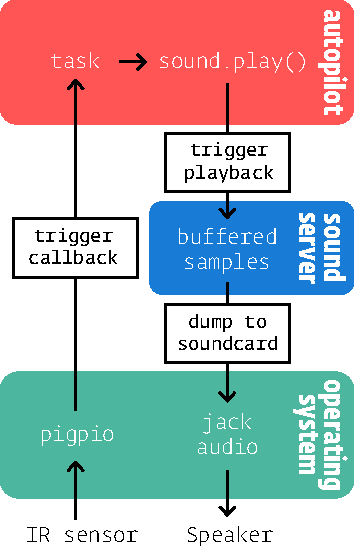
\includegraphics[]{figures/side_19_soundpath.pdf}
\caption{Our sound server keeps audio samples buffered until a \texttt{.play()} method is called, and then dumps them directly into the jack audio daemon.}
\label{fig:soundpath}
\end{marginfigure}

We use the \href{https://www.hifiberry.com/shop/boards/hifiberry-amp2/}{Hifiberry Amp 2}, a combined sound card and amplifier, which is capable of 192kHz/24Bit audio playback. Autopilot and Jack can output to any sound hardware, however, including the builtin audio of the Raspberry Pi if fidelity isn't important. There are no external video cards for the Raspberry Pi 4b\sidenote[][0cm]{though the Raspberry Pi compute module has a \href{https://web.archive.org/web/20220506011247/https://www.jeffgeerling.com/blog/2020/external-gpus-and-raspberry-pi-compute-module-4}{PCI lane that supports GPUs}.}, but its embedded video card is capable of presenting video and visual stimuli (Section \ref{sec:gonogo}) especially if the other computationally demanding parts of the task are distributed to other Raspberry Pis (Section \ref{sec:topology}). If greater video performance is needed, Autopilot is capable of running on typical desktops as well as other single-board computers with GPUs (as we did with the Nvidia Jetson in \citep{kaneRealtimeLowlatencyClosedloop2020a}).

